\documentclass[11pt]{article}
\usepackage{natbib}
\usepackage{array}
\usepackage{graphicx}
\usepackage{algorithm}
\usepackage{algpseudocode}
\usepackage{mathtools}
\DeclareMathOperator*{\argmax}{arg\,max}
\graphicspath{ {images/} }
\begin{document}

\title{Learning to Solve Arithmetic Word Problems Using Sentence Simplification}
\author{
	Vishal Rajpal\\
	Northeastern University\\
	rajpal.vi@husky.neu.edu\\
}
\date{}
\maketitle

\begin{abstract}
In order to respond to an arithmetic word problem correctly one needs to understand the question to an extent which allows determining the constraints. These are mostly semantic and are imposed by the question on its answer. Constraints from individual sentences suggest a mathematical operation and when the operators from these sentences are used collectively the answer can be derived. To extract the constraints efficiently, a concept of Syntactic Pattern is introduced which is generated by parsing the sentence using a dependency parser. It encapsulates all the relevant information in a sentence including the subject, verb and object with its quantity. Another important method for this thesis which relies on syntactic patterns is Sentence Simplification. The idea is to have a subject, verb, an object and other necessary parts of speech in the sentence so that it suggests a single operation. Based on the identified patterns a sentence may be simplified to multiple sentences. This would make the classification process easier since the sentences are less complex. To this end, it would be the classifier's job to classify the sentence to a mathematical operator. The identified operators for individual sentences are used to build a mathematical equation for the entire word problem. The results based on 3 datasets are reported and seem promising as compared to the existing systems.
\end{abstract}

\section{Introduction}
Answering arithmetic word problems has gained a lot of interest in recent years. The problem is attractive to NLP since the text is concise and relatively straightforward with identifiable semantic constraints. As these problems are directed towards elementary school students, they begin by describing a partial world state, followed by simple quantified updates or elaborations and end with a quantitative question. This information can be mapped to basic operations(addition, subtraction, multiplication and division) and an equation can be created corresponding to the problem text. 

There have been a number of attempts to solve arithmetic word problems through Machine Learning. 
All the approaches which are not template based \citep{ARIS}, \citep{RoyTACL15} and \citep{RoyR15} use different methods to extract similar information. Based on different ways the information is represented, an equation is built for the problem text. The template based method of \citep{Kushman} implicitly assumes that the solution will be generated from a set of predefined equation templates. Some of these methods only solve addition and subtraction problems \citep{ARIS}, \citep{RoyTACL15} while \citep{RoyR15} and \citep{Kushman} can solve problems for all operations.

The approach presented in this thesis can solve a general class of addition and subtraction arithmetic word problems without any predefined equation templates. In particular, it can handle an arithmetic problem as shown in Table 1.

\begin{table}[h!]
\centering
\begin{tabular}{ | m{25em} | }
\hline
Example 1:\\
\hline
For Halloween, Debby and her sister combined the candy they received. Debby had 32 pieces of candy while her sister had 42. If they ate 35 pieces the first night, how many pieces do they have left?\\
\hline
\end{tabular}
\caption{Example Arithmetic Word Problem.}
\label{table:1}
\end{table}

To derive the solution to this problem, the approach needs to understand that \textit{they} refers to \textit{Debby and her sister}. Hence, the number of candies need to be summed up and then \textit{35 candies} need to be subtracted from the total number of candies. 

While a solution to these problems requires extracting information and composing numeric expressions, if the sentence is too complex it is hard to extract information accurately.

At the heart of the technical approach, the novel notion of \textit{Sentence Simplification} is involved. Once the sentences in the problem text are simplified, extracting information becomes easier. Each sentence in the problem is simplified to a level where it consists information which is able to be mapped to a single operator. This allows us to decompose the entire problem to a collection of simplified sentences as operator prediction problems. Each sentence represents the quantitative information with the mapped operator. These predictions(operators with the quantitative information) can be combined together to form a mathematical equation.

The approach focuses on addition and subtraction problems currently, but learning to classify operators will allow us to generalize the approach to multiplication and division problems as well. In particular, the system was able to solve Example 1 although it had never seen the problem before and required both addition and subtraction operations.

The approach is evaluated on 3 datasets, achieving competitive performance on all of them. The next section describes the related work in the area of automated arithmetic word problem solving. The theory of sentence simplification is then presented. Later the information decomposition strategy that is based on it is discussed. Section 4 presents the overall computational approach, including the way classifier learns to classify simplified sentences to operators. Finally, experimental study is discussed followed with a conclusion.

\section{Related Work}
Most of the previous work in automated arithmetic problem solvers has focused on a restricted subset of problems.The approach described in \citep{RoyTACL15} handles problems with all basic operations but makes assumptions about the number of quantities in the problem text and the number of steps required to solve the problem. In contrast, our approach does not make any assumptions about the data in the problem text. Kushman's approach \citep{Kushman} tries to map numbers from the problem text to predefined equation templates and implicitly assume that similar equation forms have been seen in the training data. On the contrary, our system does not rely on pre-defined templates and hence is able to solve questions of type which have never been seen before.  The approach described in \citep{ARIS} might be the most related to ours. It handles addition and subtraction problems and tries to predict an operator for the verb in the problem text. Hence, it requires additional annotated data for verb categories. Our approach uses the information of the verb present in the sentence and handles addition and subtraction problems for now, but there is no requirement of additional annotated data. Refer to Section 5 for how the information from verbs is used as a feature. 

Most of the methods mentioned above are able to solve problems with all basic operations but our approach is easily generalizable to all the operators and also it performs competitevely compared to all other approaches. 

\section{Arithmetic Problem Representation}

Our approach addresses word problems that include addition and subtraction operations. Given a problem text, multiple fragments are extracted from it  where each fragment is a simplified version of the information presented in the sentence. We refer to these fragments as simplified sentences. Each fragment is represented based on the Parts of Speech it contains. Below are the parts of speech we consider in our representation:


\textbf{Adjective:} A problem text might have multiple types of same entities. Consider the below example:

 \begin{table}[h!]
\centering
\begin{tabular}{ | m{25em} | }
\hline
 \textbf{A pet store had 13 siamese cats and 5 house cats.}\\
\hline
 siamese cats\\
\hline
house cats.\\
\hline
\end{tabular}
\caption{Entities with Adjective.}
\label{table:2}
\end{table}

Though the example sentence has cats as the noun, but based on the adjectives\textit{(siamese and house)} there were siamese cats and house cats.
\vspace{4mm}

\textbf{Cardinal:} Cardinals are the numbers present in the problem text. We associate them to nouns based on the index at which they occur. Mostly, they occur before the noun and hence associating it is not difficult. Sometimes, the cardinal is a reference to an already occured noun. Consider the example below:

\begin{table}[h!]
\centering
\begin{tabular}{ | m{25em} | }
\hline
\textbf{He bought 2 games from a friend and bought 5 more at a garage sale.}\\
\hline
2 games\\
\hline
5 games\\
\hline
\end{tabular}
\caption{Entity with Cardinal Numbers.}
\label{table:3}
\end{table}

\textit{5 more} in the above example refers to games. We associate this to the last quantified noun encountered in the sentence.
\vspace{4mm}

\textbf{Conjunction:} Conjunctions are stored mainly to simplify the sentence. Most importantly, the index at which it occurs in the sentence plays a crucial role in creating simplified sentences.
\vspace{4mm}

\textbf{Determiner:} Determiner by definition is \textit{a modifying word that determines the kind of reference a noun or a noun group has.} 

\begin{table}[h!]
\centering
\begin{tabular}{ | m{25em} | }
\hline
\textbf{There are 28 students and every student has their own lunchbox.}\\
\hline
\textit{Every} is a determiner\\
\hline
\end{tabular}
\caption{Sentence with Determiner.}
\label{table:4}
\end{table}

In the above example, \textit{Every} is a determiner and when considering it, our system will be able to extract the information that there are \textit{28 lunchboxes}.
\vspace{4mm}

\textbf{Existential/Expletive:} Since, existentials indicate the existence or presence of something, they are an important part of speech for our system. Also, when the sentences are simplified, the existentials are added to the fragments which don't have them. Refer to the next section for more details.

\begin{table}[h!]
\centering
\begin{tabular}{ | m{25em} | }
\hline
\textbf{There are 11 rulers and 34 crayons in the drawer.}\\
\hline
There are 11 rulers in the drawer.\\
\hline
There are 34 crayons in the drawer.\\
\hline
\end{tabular}
\caption{Simplified sentences based on Existential.}
\label{table:5}
\end{table}

After the split based on conjunction \textit{and} the expletive \textit{There} is added to the fragment after the conjunction.
\vspace{4mm}

\textbf{Noun:} Nouns are important for answering the arithmetic word problems. Each problem text has some nouns in form of a subject \textit{(acting entity)} or an object \textit{(Entity that is acted upon by the subject)}. All the nouns are extracted from the simplified sentence and stored as a list. 
\vspace{4mm}

\textbf{Preposition:} Prepositions are helpful to keep track of location or time. Also, when simplifying sentences based on conjunctions we add prepositions to the fragments which are missing them. Refer to the next section for more details and example.
\vspace{4mm}

\textbf{Verb:} Verbs are important for out system to predict the type of action taken by the subject. Determining the kind of action helps to predict an operation. More details on this in Section Features.
\vspace{4mm}

\textbf{WHAdverb:} Existence of a WHAdverb mostly indicates the beginning of a question. Hence, having the WHAdverb in our representation helps us in the classification process. Refer to the Section Features.

\section{Sentence Simplification and Problem Decomposition}
Sentences in an arithmetic word problem are sometimes complex. Hence, it is difficult to extract information from such sentences. Even more challenging is to predict the impact of the sentence on the result. 

\begin{table}[h!]
\centering
\begin{tabular}{ | m{25em} | }
\hline
Example 2:\\
\hline
Henry had 11 dollars. For his birthday he got 18 more dollars but spent 10 on a new game. How much money does he have now?\\
\hline
\end{tabular}
\caption{Example Arithmetic Word Problem.}
\label{table:6}
\end{table}

The second sentence in the above example is complex for a machine learning algorithm. It has addition and subtraction operation in a single sentence. Our idea is to simplify the sentence to multiple simple sentences so that each simplified sentence has a single operation. Below are the simplified sentences for the second sentence in the above example:

\begin{table}[h!]
\centering
\begin{tabular}{ | m{25em} | }
\hline
 \textbf{For his birthday he got 18 more dollars but spent 10 on a new game.}\\
\hline
 For his birthday he got 18 more dollars.\\
\hline
He spent 10 dollars on a new game.\\
\hline
\end{tabular}
\caption{Simplified Sentences.}
\label{table:7}
\end{table}

We create a mapping for each sentence in the problem text to its simplified sentences by extracting their relational dependencies for each sentence from the stanford dependency parser\footnote{http://stanfordnlp.github.io/CoreNLP/ }. Currenly, our simplification system simplifies sentences based on conjunctions and commas. There are certain rules when simplifying the sentence.

\subsection{Rules for simplifying sentences based on conjunctions.}
 When a conjunction is encountered, our simplification system attempts to create two simplified sentences from the actual sentence. The first sentence is the part before the conjunction while the second sentence is the part after the conjunction.

But, after the split there may be some words which would be required in the second sentence. Consider the example in Table 4:

\begin{table}[h!]
\centering
\begin{tabular}{ | m{25em} | }
\hline
 \textbf{Example Sentence.}\\
\hline
The school cafeteria ordered 42 red apples and 7 green apples for students lunches.\\
\hline
\end{tabular}
\label{table:8}
\end{table}

In the sentence above, the split based on conjunction \textit{and} will result in the first sentence with a subject while the second will not have a subject and a verb. Hence, there are some rules for adding words to the second simplified sentence.

\subsubsection{Rules for adding words to second simplified sentence.}
\begin{enumerate}
 \item 
If the first sentence starts with an existential and the second does not, add the existential to the second sentence as well.

\item 
If the first sentence starts with an existential and has a verb after it, If the second sentence does not have either expletive or verb, add them to the second sentence. Consider the below example:

\begin{table}[h!]
\centering
\begin{tabular}{ | m{25em} | }
\hline
 \textbf{There were 2 siamese cats and 4 house cats.}\\
\hline
There were 2 siamese cats.\\
\hline
There were 2 house cats.\\
\hline
\end{tabular}
\caption{Example sentence for this rule.}
\label{table:9}
\end{table}

The expletive and verb were added to second sentence based on the simplification rule mentioned above.

\item
If the first sentence starts with a noun, and if the second sentence starts with a verb, the noun from the first sentence will be added to the second.

\begin{table}[h!]
\centering
\begin{tabular}{ | m{25em} | }
\hline
 \textbf{Joan ate 2 oranges and threw 3 apples.}\\
\hline
Joan ate 2 oranges.\\
\hline
Joan threw 3 apples.\\
\hline
\end{tabular}
\caption{Example sentence for this rule.}
\label{table:10}
\end{table}

\item 
If the first sentence starts with a noun and the second sentence has a \textit{noun verb} pattern, do nothing.

\begin{table}[h!]
\centering
\begin{tabular}{ | m{25em} | }
\hline
 \textbf{Tom has 9 yellow balloons and Sara has 8 yellow balloons.}\\
\hline
Tom has 9 yellow balloons.\\
\hline
Sara has 8 yellow balloons.\\
\hline
\end{tabular}
\caption{Example sentence for this rule.}
\label{table:11}
\end{table}

No words from the first sentence were added to the second since the second sentence had the \textit{noun verb (Sara has)} pattern.

\item
If the second sentence contains a preposition at the end and the first sentence does not have a preposition, the preposition from the second sentence will be added to the first. Consider the below example:

\begin{table}[h!]
\centering
\begin{tabular}{ | m{25em} | }
\hline
 \textbf{Joan found 6 seashells and Jessica found 8 seashells on the beach.}\\
\hline
Joan found 6 seashells on the beach.\\
\hline
Jessica found 8 seashells on the beach .\\
\hline
\end{tabular}
\caption{Example sentence for this rule.}
\label{table:12}
\end{table}

After splitting the sentence based on \textit{and} the preposition and the words after it \textit{on the beach} were added to the first sentence.

\item
Based on the output by the dependency parser and our rules, there might be some words which might not have been identified. But we still need those words in the simplified sentences.

\item
Therefore, the sentence simplification system identifies all the words which were not identified by our process. The words which appear before the conjunction are added to the first sentence at the right index. If the words appear after the conjunction, they are added to the second sentence.

\begin{table}[h!]
\centering
\begin{tabular}{ | m{25em} | }
\hline
 \textbf{He went to the orchard and picked peaches to stock up .}\\
\hline
Tom has 9 yellow balloons.\\
\hline
Sara has 8 yellow balloons.\\
\hline
\end{tabular}
\caption{Example sentence for this rule.}
\label{table:13}
\end{table}

\end{enumerate}

\subsection{Syntactic Pattern}
In this thesis, a new concept known as Syntactic Pattern is introduced which is basically a summarized information about a fragment. It is a pattern consisting of the initials of the parts of speech which appear in the fragment. The initials are arranged in the order in which the words appear in the sentence. Consider the below figure:

\begin{figure}[h!]
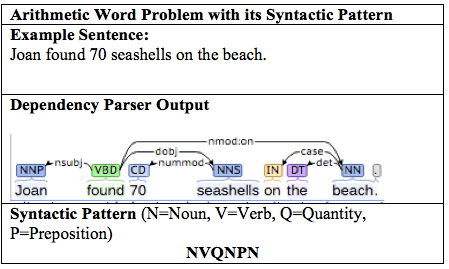
\includegraphics[width=0.9\textwidth]{Figure1}
\centering
\caption{\label{fig:Figure1}Example sentence of a word problem and its syntactic pattern.}
\end{figure}

As in the above example, the pattern \textit{NVQNPN} consists of the initials of the parts of speech in the sentence in their appearance order. This pattern is helpful in many ways:

\textbf{Grouping Multiple Fragments:} Many fragments will have a similar syntactic pattern. Our findings suggest that the fragments having a similar pattern perform similar type of operation. Refer to the below example:

\begin{table}[h!]
\centering
\begin{tabular}{ | m{16em} | m{6em} | m{6em} |}
\hline
\textbf{Example Sentence} & \textbf{Syntactic Pattern} & \textbf{Operation}\\
\hline
Joan found 70 seashells on the beach. & \textbf{NVQNPN} & Addition \\
\hline
Mary took 10 rulers from the drawer. & \textbf{NVQNPN} & Subtraction\\
\hline
Dave gave some rulers to Mary. & \textbf{NVDNPN} & Assignment\\
\hline
\end{tabular}
\caption{Example sentences and their Syntactic Pattern.}
\label{table:14}
\end{table}
 
The first two examples have the same pattern and hence perform a similar operation \textit{Addition and Subtraction}. The last sentence has a different pattern and performs an assignment operation which is different than the basic math operations. Refer to Section Features for more information.

\textbf{Metadata:} The pattern acts as a metadata for our fragments. Based on our representation, it is easy to determine if the fragment consists of any conjunction, quantities or any other parts of speech. This information is used in Section Features.

\section {Operator Prediction Classifier}
We train 4 Logistic Regression binary classifiers each for different operators \textit{(+, -, =, ?)}. We then use one versus all technique tocombine the results from the binary classifiers and determine, given a fragment \textit{f} from a problem text \textit{p}, which one of the operations \textit{f} is most likely to perform. Our training data consists of 350 labeled fragments. 

\subsection {Features}

\subsubsection{Syntactic Patterns}
From 350 training fragments, we were able to extract 125 syntactic patterns. This proves that multiple fragments had same patterns. We use these patterns as individual features. The pattern to which the fragment belongs is set\textit{(on)} and the other patterns are not set\textit{(off)}. We use one-hot encoding approach for pattern features.

\subsubsection{Occurence based Features}

\textbf{Relation based occurence features:} Dependency relations in a fragment depict its structure. Presence of some dependency relations is useful for the classifier to predict operations. Particularly, \textit{nmod:poss} relation if exists in the fragment, can determine information about a subject possessing an object. \textit{nmod:of} helps to differentiate between two nouns of same kind. Below are the examples:

\newpage
\begin{table}[h!]
\centering
\begin{tabular}{ | m{25em} | }
\hline
 \textbf{Sam had 20 pieces of cake and 10 pieces of butter in his plate.}\\
\hline
\textit{nmod:of(pieces-4, cake-6)}\\
\hline
\textit{nmod:of(pieces-9, butter-11)}\\
\hline
\textit{nmod:poss(plate-14, his-13)}\\
\hline
\end{tabular}
\caption{Example relations in the fragment.}
\label{table:16}
\end{table}

As in the above example, it is easy to see that presence of these relations is mostly in the fragments in which some operation takes place.

\textbf{Pattern based occurence features:} Occurence of some sprecific sub pattern in the syntactic pattern of the fragment can be helpful. Specifically, \textbf{NVQN} and \textbf{QN} are used as features for the classifier. Their presence again indicates some operation. Consider the below example:

\begin{table}[h!]
\centering
\begin{tabular}{ | m{20em} | m{5em} |}
\hline
 \textbf{Sentence} & \textbf{Syntacttic Pattern}\\
\hline
George had 30 dollars. & \textbf{NVQN} \\
\hline
18 cupcakes were sold. & \textbf{QNVV} \\
\hline
\end{tabular}
\caption{Example occurence of a sub pattern.}
\label{table:17}
\end{table}

In the first exmaple, both \textit{NVQN} and \textit{QN} appear. While, in the second \textit{QN} appears. Presence of quantity in a fragment is more likely to suggest an operation. 

\textbf{Word based occurence features:} Occurence of some particular words in the fragment help the classifier. Below is list of some words and description of how they are helpful:

\begin{table}[h!]
\centering
\begin{tabular}{ | m{5em} | m{15em} | m{15em} | }
\hline
 \textbf{Word} & \textbf{Description} & \textbf{Example}\\
\hline
\textit{now} & Suggests a resulting output after some operations. & 28 students wanted to have fruit. There are now 12 fruits remaining. \\
\hline
\textit{most, several, some} & Suggest an unknown quantity in the fragment. & Joan gave some of her seashells to Sam. \\
\hline
\end{tabular}
\caption{Examples for occurence of specific words.}
\label{table:17}
\end{table}

\subsubsection{Count based Features}
Based on our analysis we found that having a count of some parts of speech occuring the the syntactic pattern proves to be helpful to the classifier in learning accurately. Refer to Table 14 for more details:

\begin{table}[h!]
\centering
\begin{tabular}{ | m{5em} | m{25em} |}
\hline
\textbf{Feature} & \textbf{Description} \\
\hline
 Number of Nouns. & Generally a fragment having 2 nouns\textit{subject and object} is more likely to be predicted to addition or subtraction operation.\\
\hline
Number of Prepositions. & A single preposition(such as \textit{from} or \textit{to} is suggesting some basic math operation.\\
\hline
Number of Verbs. & This is basically to indicate that of a verb exists, the fragment suggests an operation.\\
\hline
Number of Quantities. & Similar to verbs, existence of quantities in the fragment is more likely to predict an operation.\\
\hline
\end{tabular}
\caption{Count based Features.}
\label{table:15}
\end{table}

\subsubsection{Verb similarity based features}
Verbs are important to determine the kind of action the fragment is trying to perform. The verbs present in the sentence are given as an input to WordNet\textit{(a large lexical database of English. Nouns, verbs, adjectives and adverbs are grouped into sets of cognitive synonyms)} and Word2Vec\textit{Computes vector representations of words}. 

For an input verb \textit{v}, WordNet outputs a set of categories \textit{($c_{1}$, $c_{2}$,...,$c_{n}$)} to which the verb is most likely to belong. We shortlisted 8 verb categories which can prove helpful to our system. 

\begin{table}[h!]
\centering
\begin{tabular}{ | m{15em} | }
\hline
 \textbf{Verb Categories.}\\
\hline
verb.possession\\
\hline
verb.change\\
\hline
verb.communication\\
\hline
verb.consumption\\
\hline
verb.contact\\
\hline
verb.creation\\
\hline
verb.motion\\
\hline
verb.weather\\
\hline
\end{tabular}
\caption{Shortlisted Verb Categories.}
\label{table:18}
\end{table}

We use Word2Vec to get 3 nearest words to the verb and send those words as an input to WordNet to get the verb categories they belong. We normalize the results for these 3 words and the results for the verb itself. Hence, In total we have 8 normalized similarity based features(verb categories)

\subsection{Logistic Regression Classifier}

Logistic Regression tries to fit a model of the form \begin{math} p(y|X) \end{math} which directly models the mapping from input \begin{math}X\end{math} to output \begin{math}y\end{math}. Since, it discriminates between class labels it is known as a discriminaive classifier. LR corresponds to following binary classification model:

\begin{equation} p(y|X,W) = Ber(y|sigm(W^{T}X)) \end{equation}

Each fragment will to be classified to one of the operators/class mentioned in the below table:

\begin{table}[h!]
\centering
\begin{tabular}{ | m{5em} | m{20em} |}
\hline
 \textbf{Operator} & \textbf{Description}\\
\hline
+ & Addition operation. \\
\hline
- & Subtraction operation. \\
\hline
= & Assignment operation. \\
\hline
? & The fragment is asking some question.\\
\hline
\end{tabular}
\caption{Logistic Regression output classes.}
\label{table:19}
\end{table}

Each class has its own binary LR classifier. We use an algorithm known as \textbf{Stochastic Gradient Descent (SGD)} to train all the four LR classifiers. Below is the algorithm:

\begin{algorithm}
\caption{Stochastic Gradient Descent (SGD)}
\textit{Initialize $\theta$, $\eta$, b;}
\begin{algorithmic}
\Repeat 
\State Randomly permute data;
\For{\texttt{i = 1:N}}
\State s = sigm($X_{i}$);
\State updateWeightVector(s, $X_{i}$);
\State g = updateGradient(s, $y_{i}$);
\State Update b;
\EndFor
\Until
\end{algorithmic}
\end{algorithm}

We have 3 parameters as shown above: $\theta$(weight vector), $\eta$(learning rate) and b(bias). In SGD, we repeatedly run through the training set, and each time we encounter a training example, we update the parameters according to the gradient of the error with respect to that single example only. We calculate the error based on sigmoid function value. A sigmoid function is a mathematical function having an \textit{S} shaped curve \textbf{sigmoid curve}. Below is the sigmoid function:

\begin{figure}[h!]
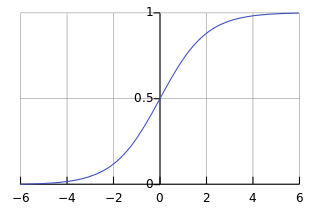
\includegraphics[width=0.7\textwidth]{Figure2}
\centering
\caption{\label{fig:Figure2}Sigmoid Curve.}
\end{figure}

The function is defined by the below formula:
\begin{flalign*}
&S(t) = \frac{1}{1 + e^{-t}} \\
&t = \theta_{T}X \\
&\theta \rightarrow Weight vector \\
&X \rightarrow Feature vector for an example
\end{flalign*}

The function has finite limits and approaches negative infinity from the left side and to infinity from the right.  When the algorithm encounters an example, it updates the weight for a particular feature in the weight vector if the feature is set in the current example's feature vector. Based on the sigmoid function value, the gradient and all the parameters are updated. 

\subsubsection{Training the classifier}
We train our four LR binary classifiers on 300 operator labeled fragments and then use one versus all\textit(OvA) technique to combine the results from all four of them. The OvA strategy involves training a single classifier per class\textit(4 operators in our case). The samples of that class are treated as positive and all other samples are treated as negative. For example, when training a classifier for \textbf{+} operator, the training samples having \textbf{+} label are positive and samples having other labels i.e. \textbf{-, =, ?} are considered negative. This strategy requires the base classifiers to produce a real-valued confidence score for its decision, rather than just a label. Once we have a real valued score from all the base classifiers, the technique predicts a single class using the below mechanism:

\begin{equation}
y^{\prime} = \argmax_{k = 1,...,K} f_{k}(x)
\end{equation}

\subsubsection{Precision and Recall}
Our testing data consists of 55 fragments. Below is the distribution of fragments among all the operations and their precision and recall values:


\begin{table}[h]
\begin{center}
\begin{tabular}{|c|c|c|c|}
\hline
\bf Operator & \bf No. of instances & \bf Precision & \bf Recall \\
\hline
+ & 32 & 95.83\% & 71.87\% \\
\hline
- & 9 & 40\% & 66.66\% \\
\hline
= & 2 & 50\% & 50\% \\
\hline
? & 15 & 82.35\% & 93.33\% \\
\hline
\end{tabular}
\end{center}
\label{table:20}
\caption{Precision and Recall}
\end{table}

The higher precision and recall of \textbf{?} is well understood as there were features such as the presence of an WHAdverb which made it easy for the classifier to predict them accurately. Whereas, for \textbf{+} the verb based similarity features played an important role. For \textbf{-} and \textbf{=} its not reallt correct to judge since there were less number of testing fragments.

\subsection{Experimental Results}
In this section, we evaluate the proposed method on publicly available datasets of arithmetic word problems. We show the parameter setup of our LR classifiers. Lastly, we evaluate the performance of the full system.

\subsubsection{Datasets}
We evaluate our system on three datasets, each of which comprise a different category of arithmetic word problems.

\begin{enumerate}
\item \textbf{A12 Dataset:} This dataset is a collection of 395 addition and subtraction problems, released by \citep{ARIS}. They perform a 3-fold cross validation, with every fold containing problems from different sources. This helps to evaluate robustness to domain diversity. To evaluate our system, we follow the same evaluation setting.

\item \textbf{IL Dataset:} This is a collection of arithmetic problems released by \citep{RoyTACL15}. Each of these problems can be solved by performaing one operation. This dataset consists of problems having all basic operations but we only consider addition and subtraction problems. Though, we cannot compare our results to them, we still achieve a competitive accuracy on addition and subtraction problems. We use a 5-fold cross validation to evaluate on this dataset.

\item \textbf{Commoncore Dataset:} This dataset is released by \citep{RoyR15} and consists of 600 word problems. These problems similar to the IL dataset have all basic operations, but we only consider addition and subtraction problems. 200 problems have addition and subtraction operations in them. We perform 6-fold cross validation to evaluate on these problems.
\end{enumerate}


\subsubsection{Experimental Setup}
\newpage
\bibliographystyle{apalike}
\bibliography{Thesis}



\end{document}